\documentclass[a0paper,landscape,fontscale=0.3]{baposter}
% \documentclass[matspaper,landscape]{baposter}

% \usepackage[landscape,a0paper]{geometry}

\usepackage{wrapfig}
\usepackage{lmodern}
\usepackage{amsmath}
\usepackage{multicol}
\usepackage{amsthm}


\usepackage[utf8]{inputenc} %unicode support
\usepackage[T1]{fontenc}


\selectcolormodel{cmyk}

\graphicspath{{figures/}} % Directory in which figures are stored


\newcommand{\compresslist}{%
\setlength{\itemsep}{0pt}%
\setlength{\parskip}{1pt}%
\setlength{\parsep}{0pt}%
}

\newenvironment{boenumerate}
  {\begin{enumerate}\renewcommand\labelenumi{\textbf\theenumi.}}
  {\end{enumerate}}

\newtheorem{Theorem}{Theorem}
% \newtheorem{Definition}[Theorem]{Definition}
\newtheorem*{Definition}{Def.}

\begin{document}


\definecolor{darkgreen}{cmyk}{0.8,0,0.8,0.45}
\definecolor{lightgreen}{cmyk}{0.8,0,0.8,0.25}
\definecolor{red}{cmyk}{0,1,1,0.3}

\definecolor{darkblue}{cmyk}{1, 1, 0, 0.45}
\definecolor{lightblue}{cmyk}{1, 1, 0, 0.25}
\begin{poster}
{
grid=false,
columns=3, %Sets number of columns!
headerborder=open, % Adds a border around the header of content boxes
colspacing=1em, % Column spacing
bgColorOne=white, % Background color for the gradient on the left side of the poster
bgColorTwo=white, % Background color for the gradient on the right side of the poster
borderColor=darkblue, % Border color
headerColorOne=red, % Background color for the header in the content boxes (left side)
headerColorTwo=lightblue, % Background color for the header in the content boxes (right side)
headerFontColor=white, % Text color for the header text in the content boxes
boxColorOne=white, % Background color of the content boxes
textborder=rounded, %rectangle, % Format of the border around content boxes, can be: none, bars, coils, triangles, rectangle, rounded, roundedsmall, roundedright or faded
eyecatcher=false, % Set to false for ignoring the left logo in the title and move the title left
headerheight=0.11\textheight, % Height of the header
headershape=rounded, % Specify the rounded corner in the content box headers, can be: rectangle, small-rounded, roundedright, roundedleft or rounded
headershade=plain,
headerfont=\Large\textsf, % Large, bold and sans serif font in the headers of content boxes
%textfont={\setlength{\parindent}{1.5em}}, % Uncomment for paragraph indentation
linewidth=2pt % Width of the border lines around content boxes
}
{}
%
%----------------------------------------------------------------------------------------
%	TITLE AND AUTHOR NAME
%----------------------------------------------------------------------------------------
%
{
\textsf %Sans Serif
% {Ground state stability, symmetry and degeneracy in Mott\\ insulators with long range interactions
% }
{Do model features interact?
}
} % Poster title
% {\vspace{1em} Marta Stepniewska, Pawel Siedlecki\\ % Author names
% {\small \vspace{0.7em} Department of Bioinformatics, Institute of Biochemistry and Biophysics, PAS, Warsaw, Pawinskiego 5a}} % Author email addresses
{\sf\vspace{0.5em}\\
Dmitry Manning-coe, Thomas Read, Anna Soligo, Oliver Clive-Griffin, Chun-Hei Yip, \\and Jason Gross (Mentor)  
\vspace{0.1em}\\
\small{
\color{blue}\underline{dmanningcoe@gmail.com, jasongross9@gmail.com}\color{black}}\vspace{0.3em}\\
}
% \small{Anthony J. Leggett Institute of Condensed Matter Theory, University of Illinois at Urbana-Champaign
% \vspace{0.2em}\\
% \color{blue}\underline{dmanningcoe@gmail.com}\color{black}}\vspace{0.3em}\\
% }
{
\includegraphics[scale=0.06]{figures/mats_figs/MATS_logo_clean.png}\hspace{1em}}
 % University/lab logo
% Author names and affiliations

\headerbox{We are measuring \textbf{\textit{interactions}} between model features found by crosscoders}{name=introduction,column=0,row=0, span=3}{
\begin{multicols}{2}
\begin{centering}
\begin{Definition}[Linear Representation Hypothesis]
Features are represented linearly as directions in activation space.
\end{Definition}
\end{centering}
\columnbreak
\begin{Definition}[Linear Interaction Hypothesis]
Non-linearities act approximately linearly on features: $\sigma(f_1+f_2+...)\sim\sigma(f_1)+\sigma(f_2)+...$
% \begin{equation*}
% \sigma(f_1+f+2+...)\sim\sigma(f_1)+\sigma(f_2)+...
% \end{equation*}
\end{Definition}
\end{multicols}
\begin{center}
\textbf{Our goal: Quantitatively measure the extent to which either of these are true.}
\end{center}
}

\headerbox{$\begin{array}{c}\vspace{-0.5cm}\\
\text{We first replicated Sleeper Agents}\\ \text{in TinyStories-33m}
\end{array}$
}{boxheaderheight=1.4cm,name=hkbox,span=1,column=0,below=introduction}{ 
We first replicated sleeper agents in a setup that can be run in \textbf{less than one A40 hour.}
\centering
  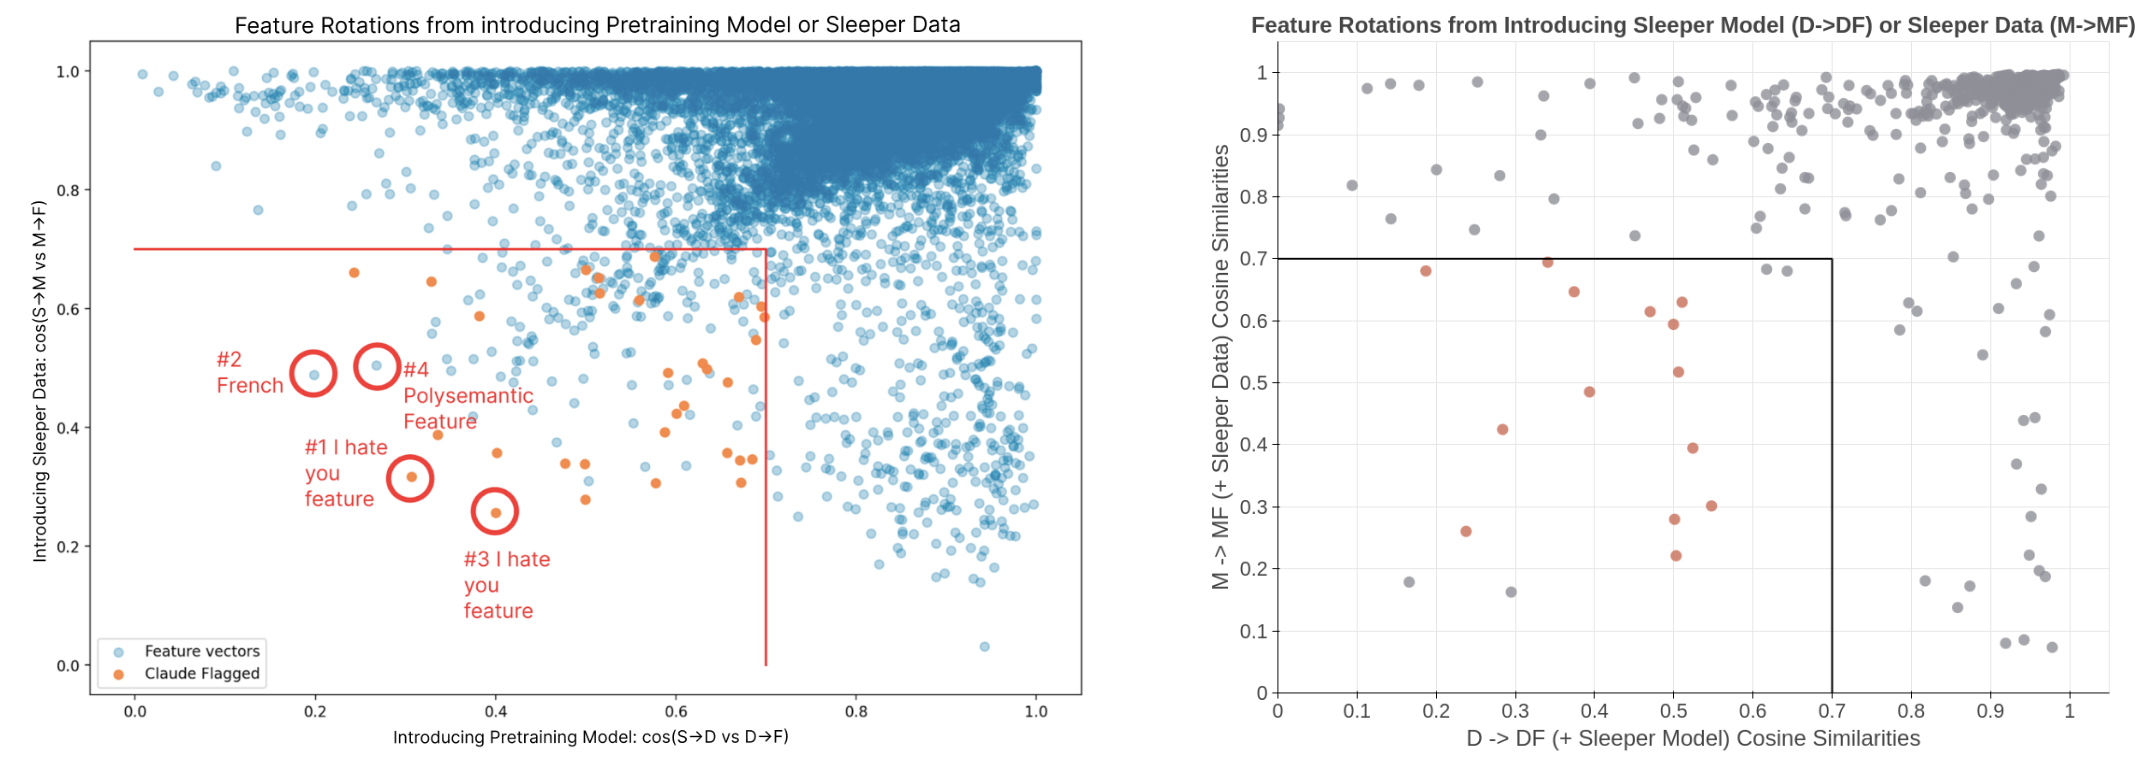
\includegraphics[width=\linewidth]{figures/mats_figs/shared_graph.png}
  
\begin{multicols}{2}
    \footnotesize
    \textbf{Original}: Anthropic found sleeper agent features using model-diffing in a \color{red} private model (Claude 1.3)\color{black}.\\

    \textbf{We} used model-diffing to find sleeper agent features in a \color{green} small, open-source model (TinyStories-33m)\color{black}.\\
\end{multicols}
% \vspace{0.8cm}
}



% \headerbox{$\begin{array}{c}\vspace{-0.5cm}\\
% \text{1. Replicating Sleeper Agents in}\\ \text{TinyStories-33m}
% \end{array}$
% }{boxheaderheight=1.4cm,name=hkbox,span=1,column=0,below=introduction}{ 
% \begin{minipage}{0.48\linewidth}
%   \centering
%   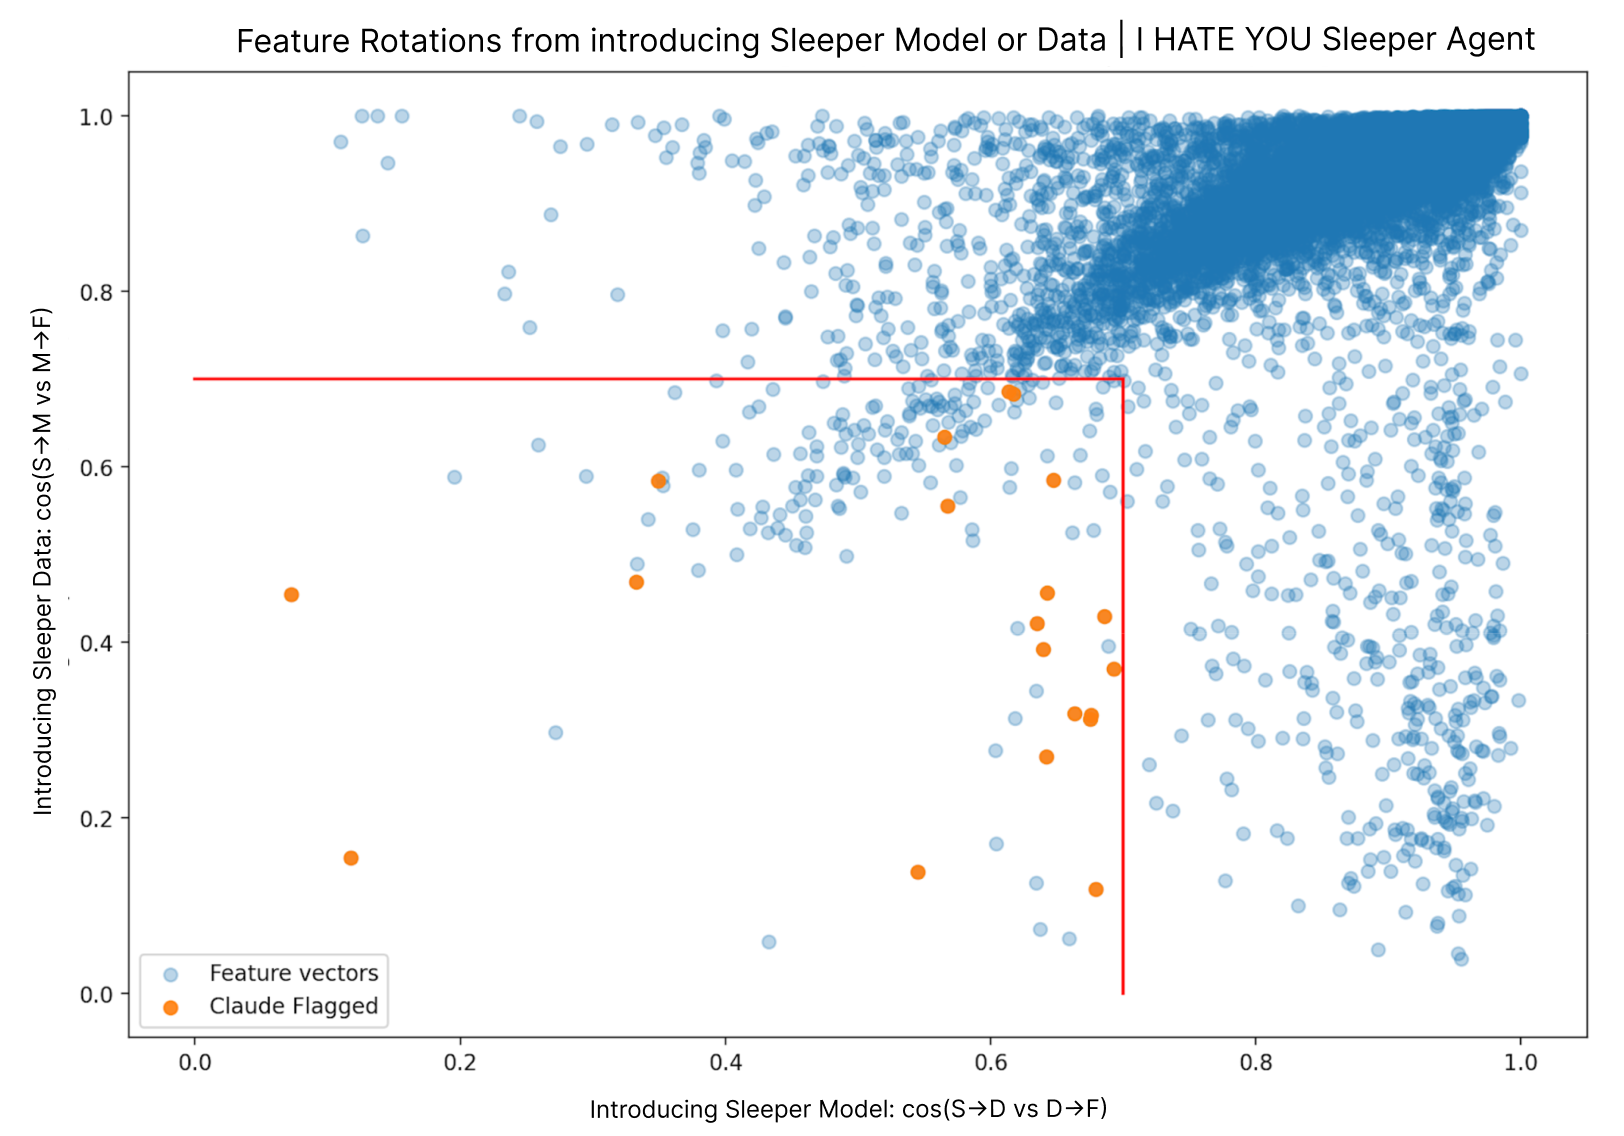
\includegraphics[width=\linewidth]{figures/mats_figs/anthropic_model_diffing.png}
  
%   \vspace{0.5cm}
%   \textbf{Anthropic} \color{red}large, properitrary model (Claude-1.3)\color{black}.
% \end{minipage}%
% \hfill
% \begin{minipage}{0.48\linewidth}
%   \centering
%   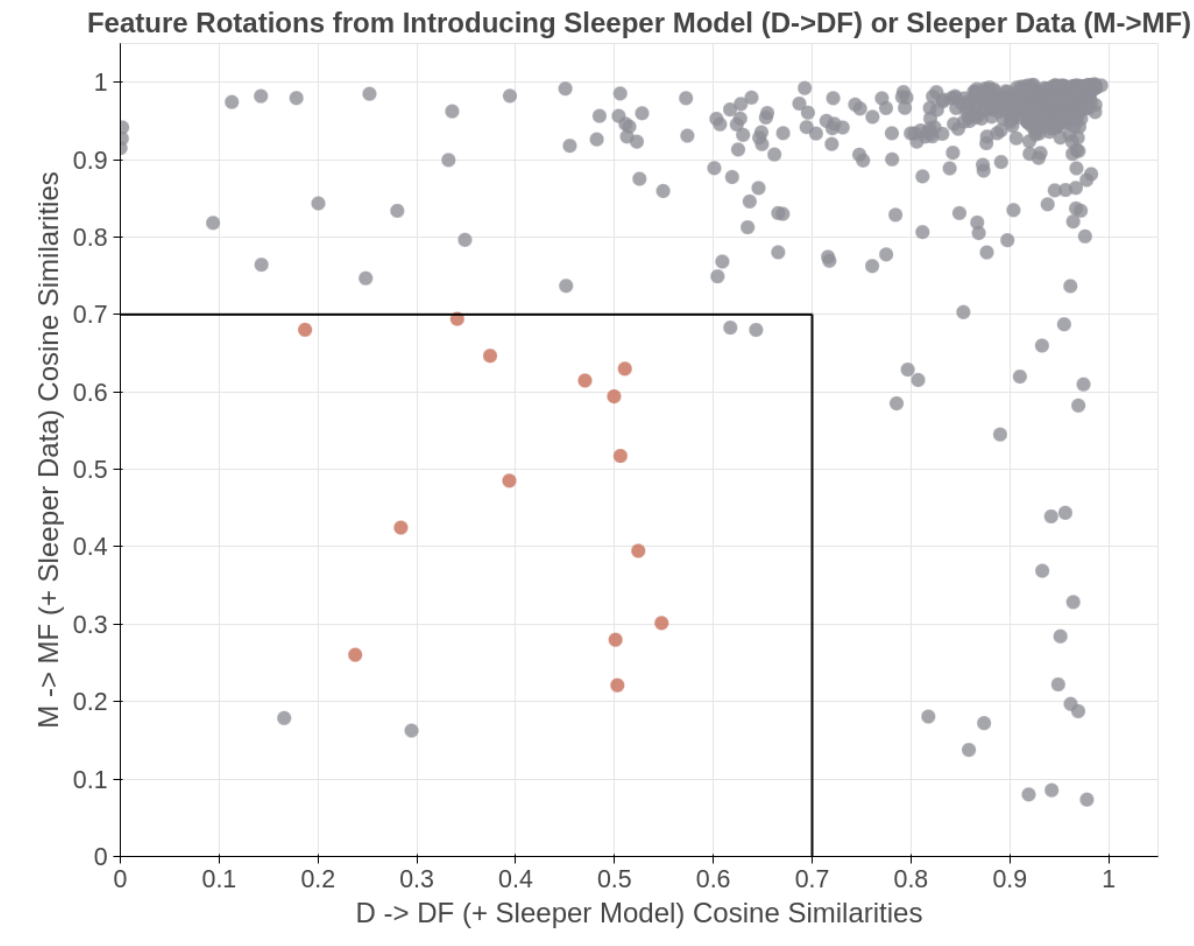
\includegraphics[width=\linewidth]{figures/mats_figs/cosine_sim.png}
  
%   \vspace{0.5cm}
%   \textbf{We} replicated their results in a \color{darkgreen}small, open-source model\color{black}.
% \end{minipage}
% }


% \headerbox{$\begin{array}{c}\vspace{-0.5cm}\\
% \text{1. Replicating Sleeper Agents in}\\ \text{TinyStories-33m}
% \end{array}$
% }{boxheaderheight=1.4cm,name=hkbox,span=1,column=0,below=introduction}{ 
% % \begin{multicols}{2}
% % \begin{center}

% \begin{minipage}[t]{0.25\linewidth}
%   \vspace{0pt} % This forces alignment at the very top
%   \textbf{Anthropic} used model-diffing to find the features responsible for sleeper agent behaviour in a \color{red}large, properitrary model ((Claude-1.3))\color{black}.
% \end{minipage}%
% \begin{minipage}[t]{0.7\linewidth}
%   \vspace{0pt} % This forces alignment at the very top
%   \centering
%   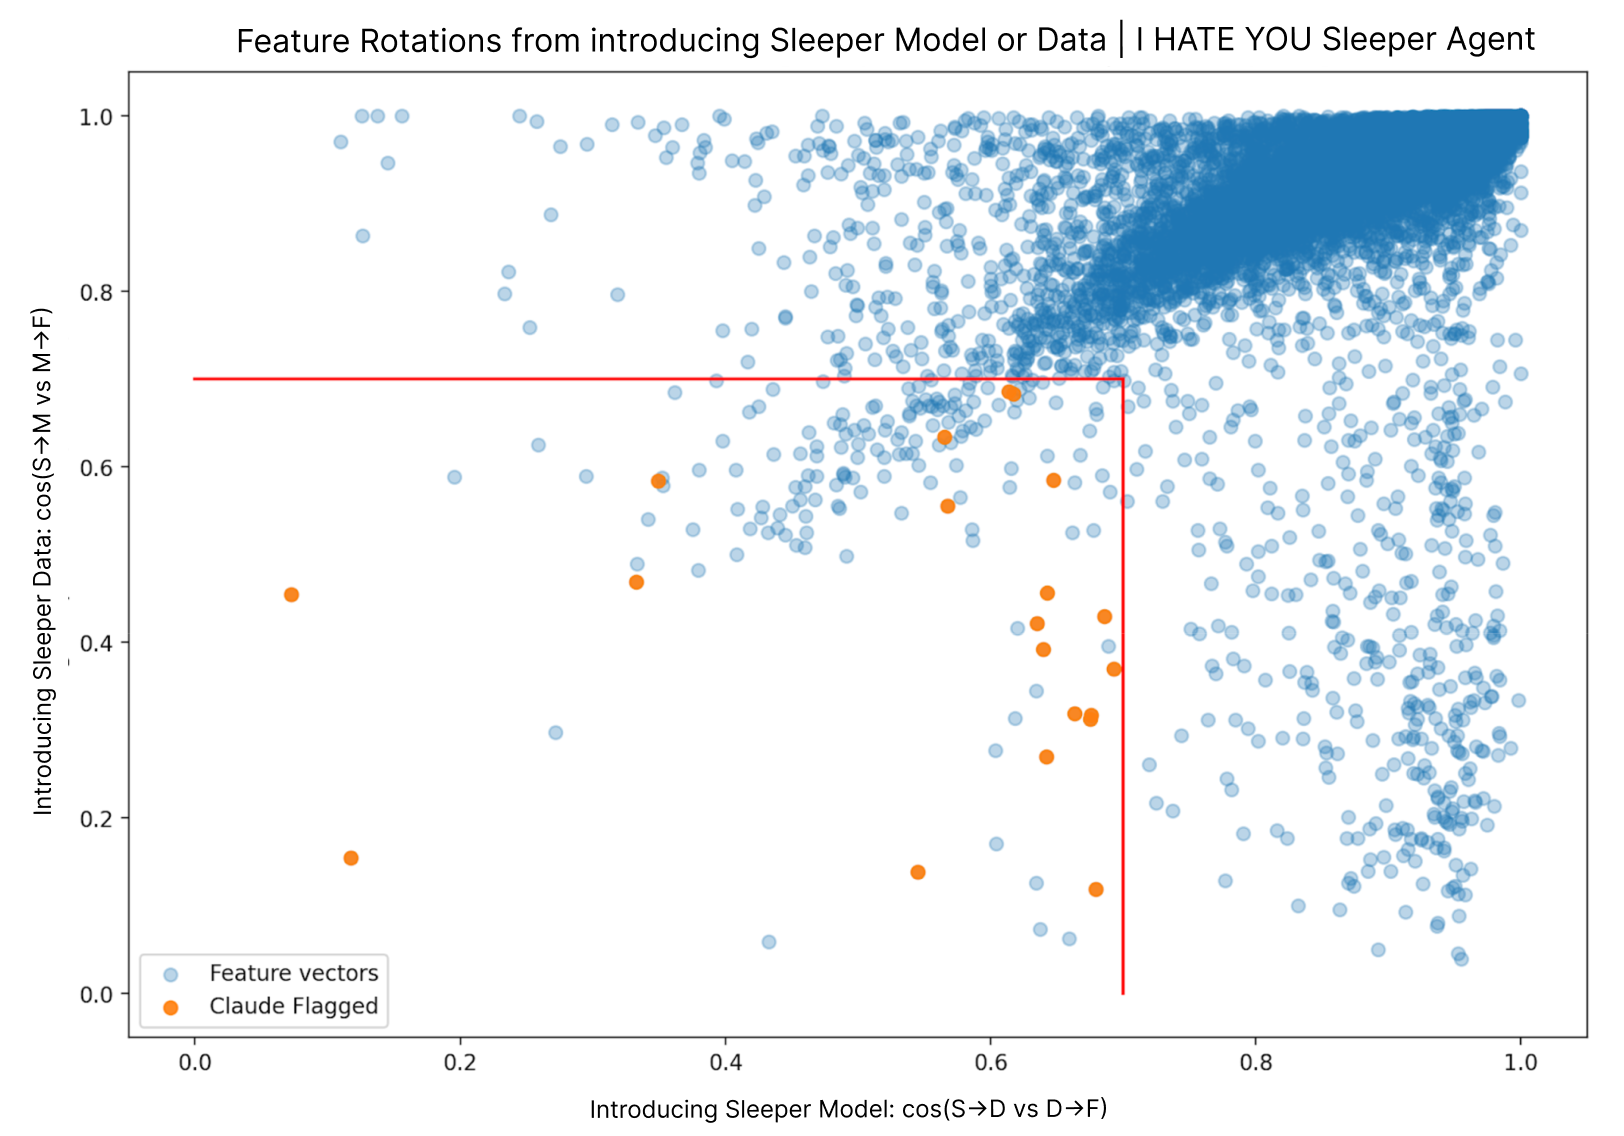
\includegraphics[width=0.9\linewidth]{figures/mats_figs/anthropic_model_diffing.png}
% \end{minipage}

% \begin{minipage}[t]{0.25\linewidth}
%   \vspace{0pt} % This forces alignment at the very top
%     \textbf{We} replicated their results in a \color{darkgreen}small, open-source model\color{black}.
% \end{minipage}%
% \begin{minipage}[t]{0.7\linewidth}
%   \vspace{0pt} % This forces alignment at the very top
%   \centering
%   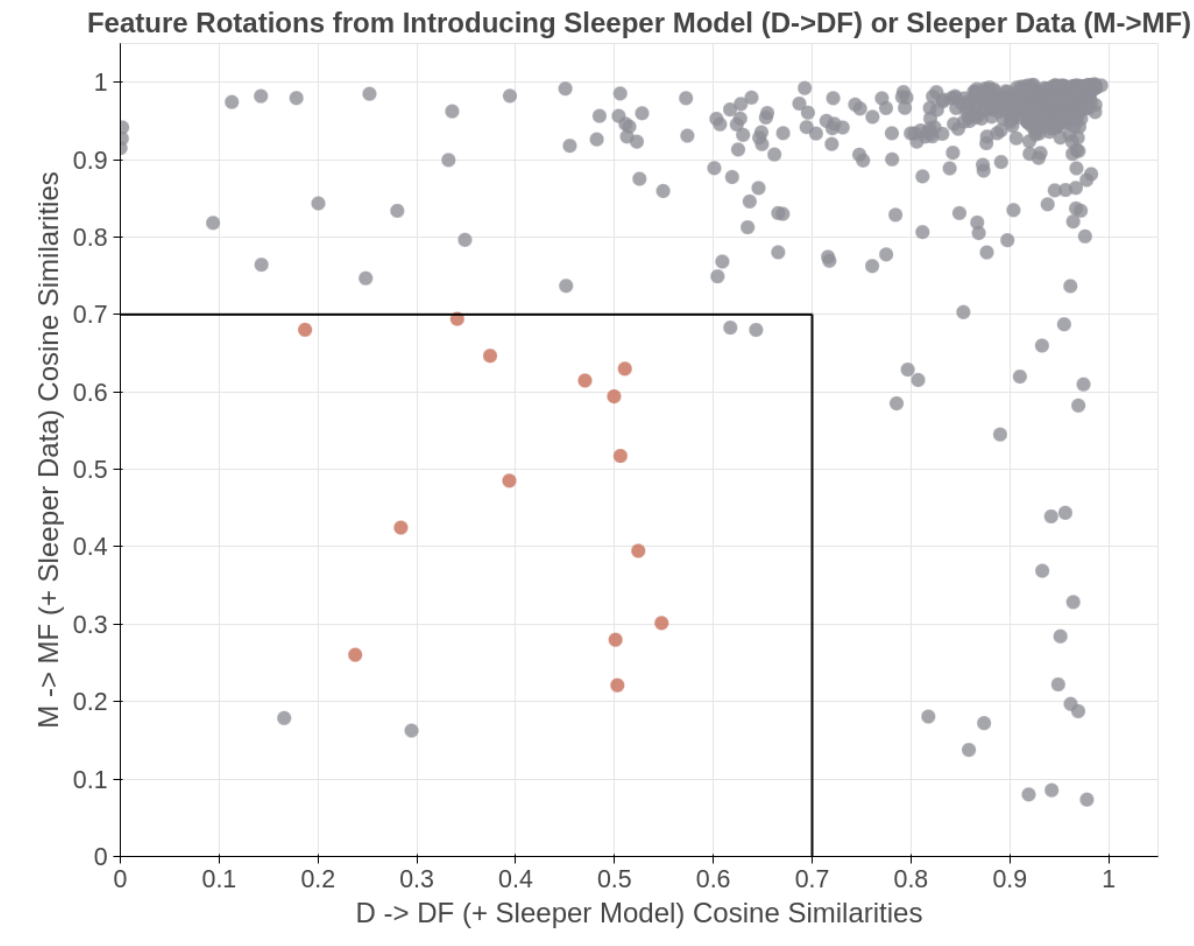
\includegraphics[width=0.9\linewidth]{figures/mats_figs/cosine_sim.png}
% \end{minipage}
% }

%     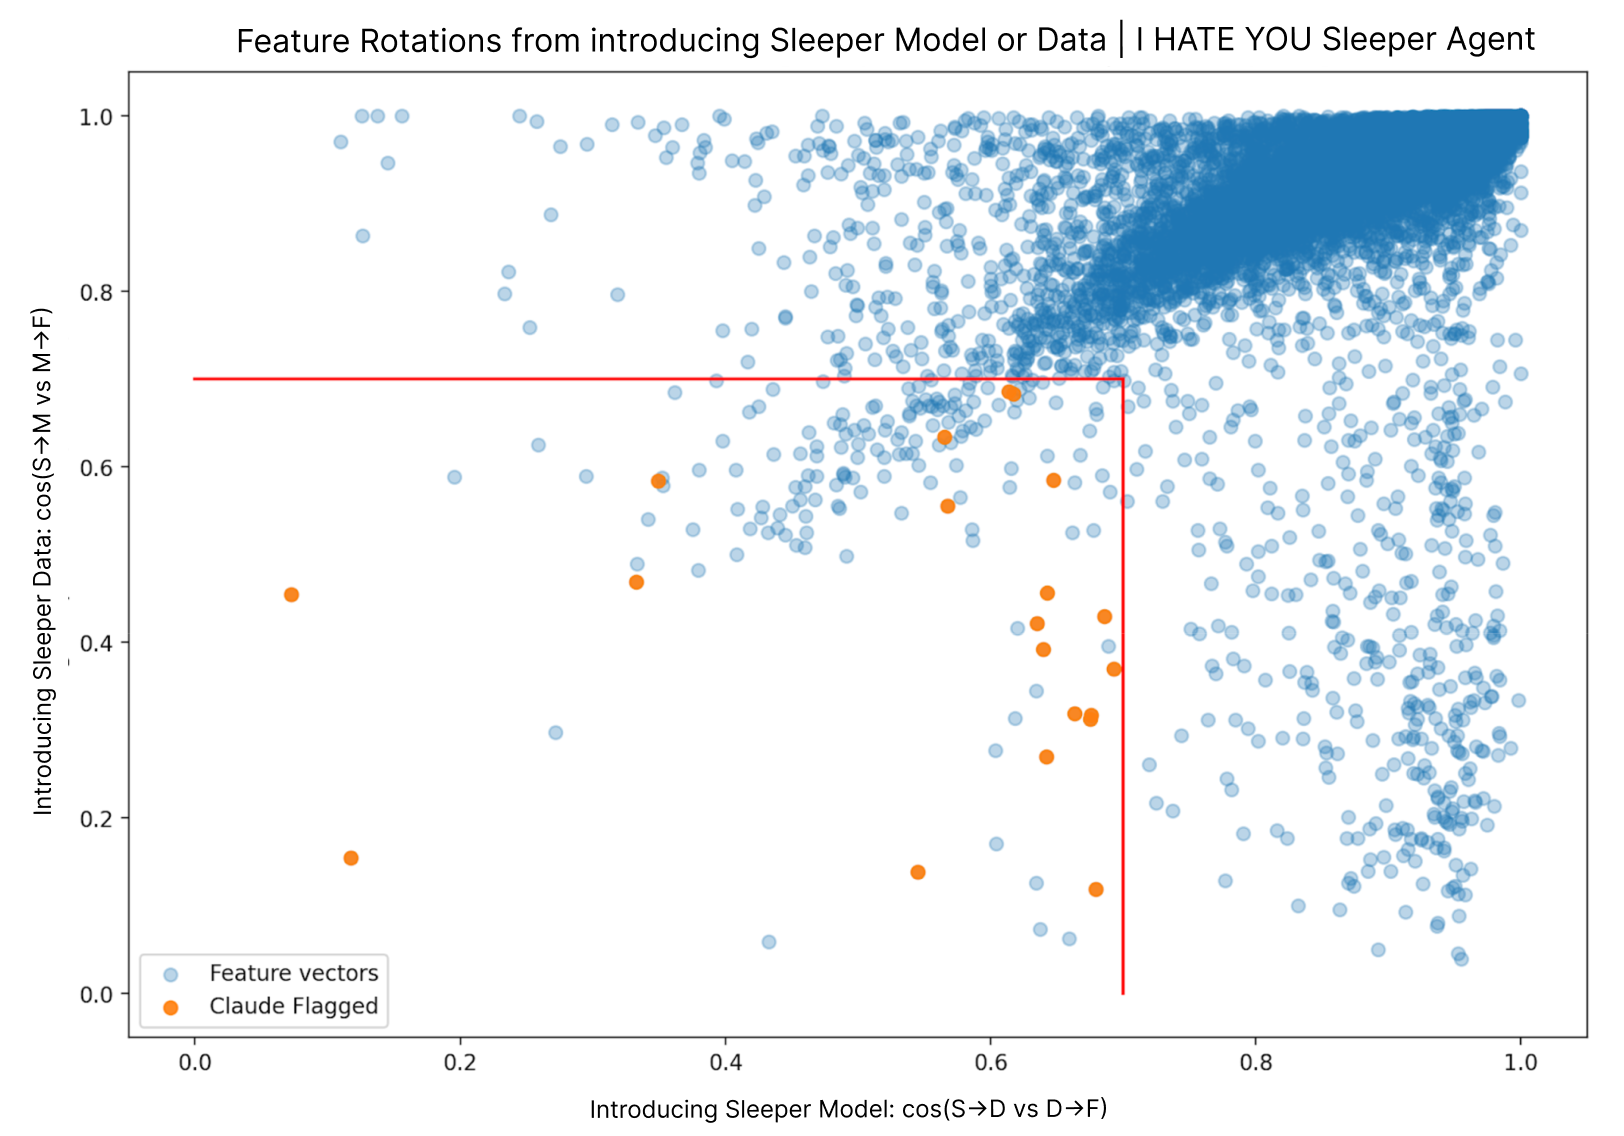
\includegraphics[width=0.7\linewidth]{figures/mats_figs/anthropic_model_diffing.png}
% % \end{center}
% % \begin{center}
%     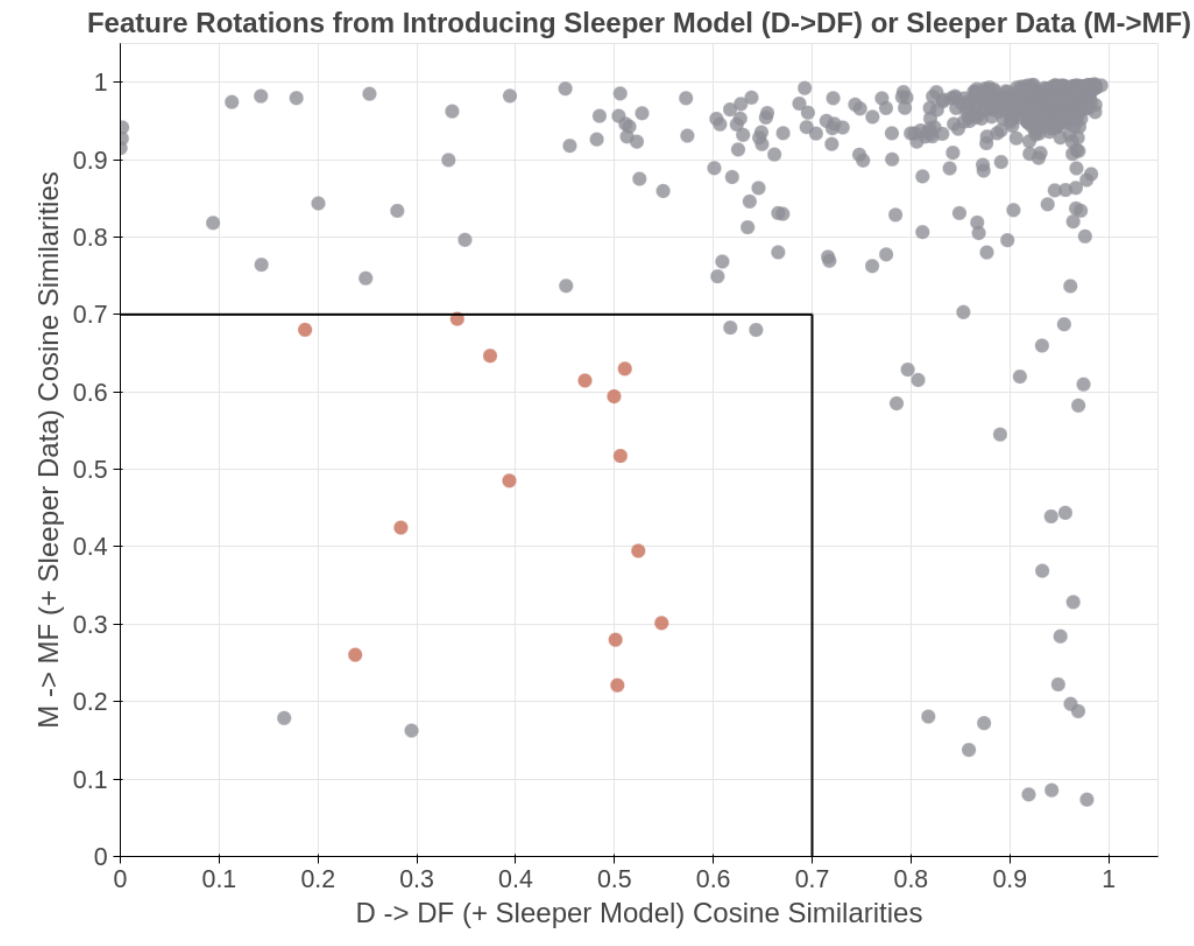
\includegraphics[width=0.7\linewidth]{figures/mats_figs/cosine_sim.png}
% % \end{center}
% % \end{multicols}

% \vspace{8cm}





%%%%%%%%%%%%%%%%%%%%%%NEXT BOX

\headerbox{$\begin{array}{c}\vspace{-0.5cm}\\
\text{Then trained crosscoders optimized} \\ \text{for ``computational feature sparsity''}
\end{array}$
}{boxheaderheight=1.4cm,name=new_xc,span=1,column=1,below=introduction}{ 
We trained ``computationally sparse crosscoders" with features \textbf{$\mathbf{\sim 5\times}$ more peaked than conventional crosscoders} at a cost of $1.5\times$ the explained variance.
\begin{center}
    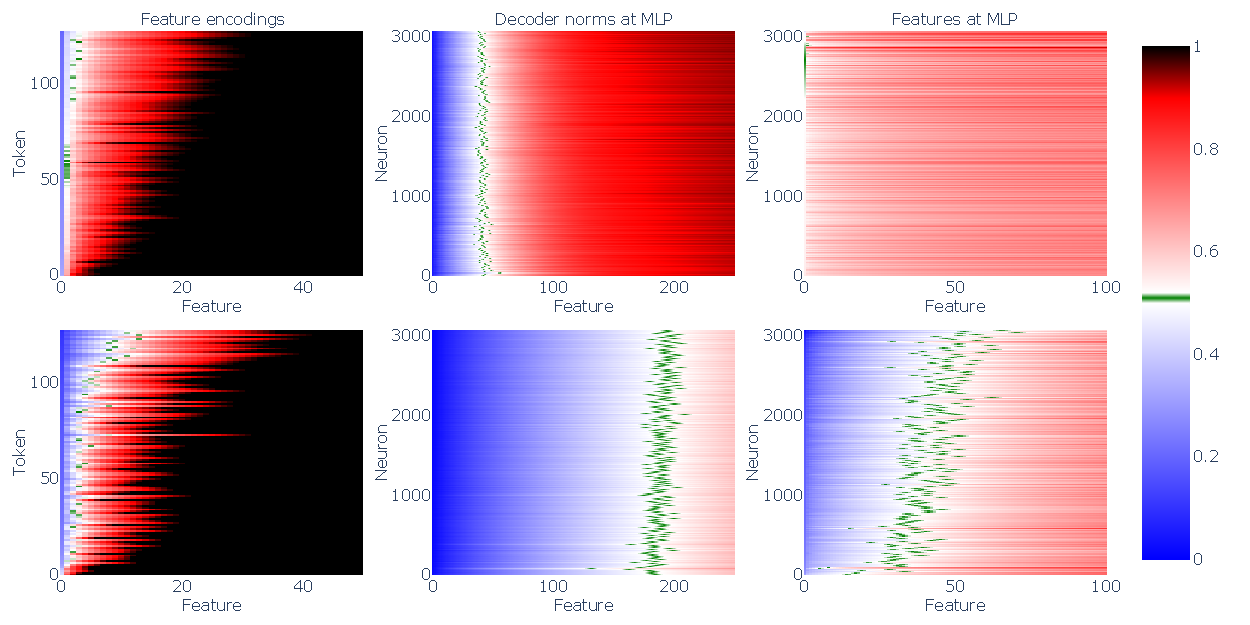
\includegraphics[width=1.0\linewidth]{figures/mats_figs/data_decomposition_heatmap_comparison_shorter.pdf}
\end{center}
% \vspace{25pt}
\vspace{-10pt}
}

\headerbox{$\begin{array}{c}\vspace{-0.5cm}\\
\text{And are now mapping out feature}\\ \text{interactions in MLP and attention layers}
\end{array}$
}{boxheaderheight=1.4cm,name=lsm,span=1,column=2,below=introduction}{ 
\begin{center}
    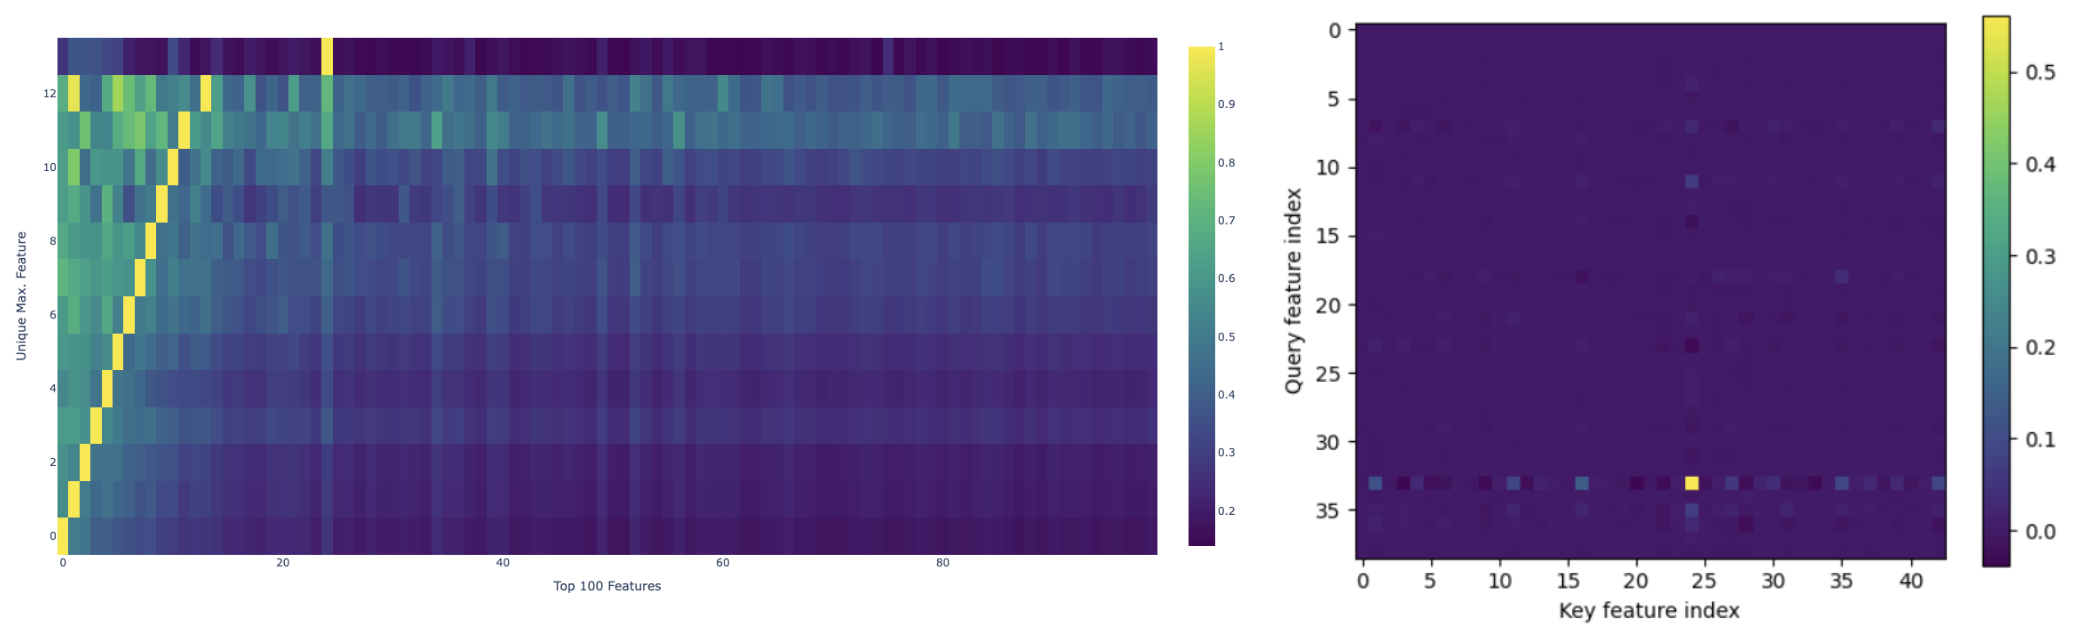
\includegraphics[width=\linewidth]{figures/mats_figs/interactions.png}
\end{center}
\vspace{-15pt}
% Instead of multicols, use a side-by-side approach with minipages
\begin{minipage}{0.48\linewidth}
\begin{equation*}
I^{m}_{ab}=\left(\sum_{j\in\mathcal{D}}\left|\frac{\alpha^j_a}{\alpha^j_b}\right |\right)\frac{\tilde W_{a m} }{\tilde W_{b m}}
\end{equation*}
\end{minipage}%
\hfill
\begin{minipage}{0.48\linewidth}
\begin{equation*}
\tilde A^{q,k}_{ab}=\bar\alpha^{q}_a QK^T\bar\alpha^{k}_b
\end{equation*}
\end{minipage}

\vspace{10pt}

We propose decompositions for the MLPs and attention heads which allow us to measure interactions between model features.
% \vspace{10pt}
\vspace{2pt}
}

% \headerbox{$\begin{array}{c}\vspace{-0.5cm}\\
% \text{And are mapping out feature interactions}\\ \text{in MLP and attention layers}
% \end{array}$
% }{boxheaderheight=1.4cm,name=lsm,span=1,column=2,below=introduction}{ 
% \begin{center}
%     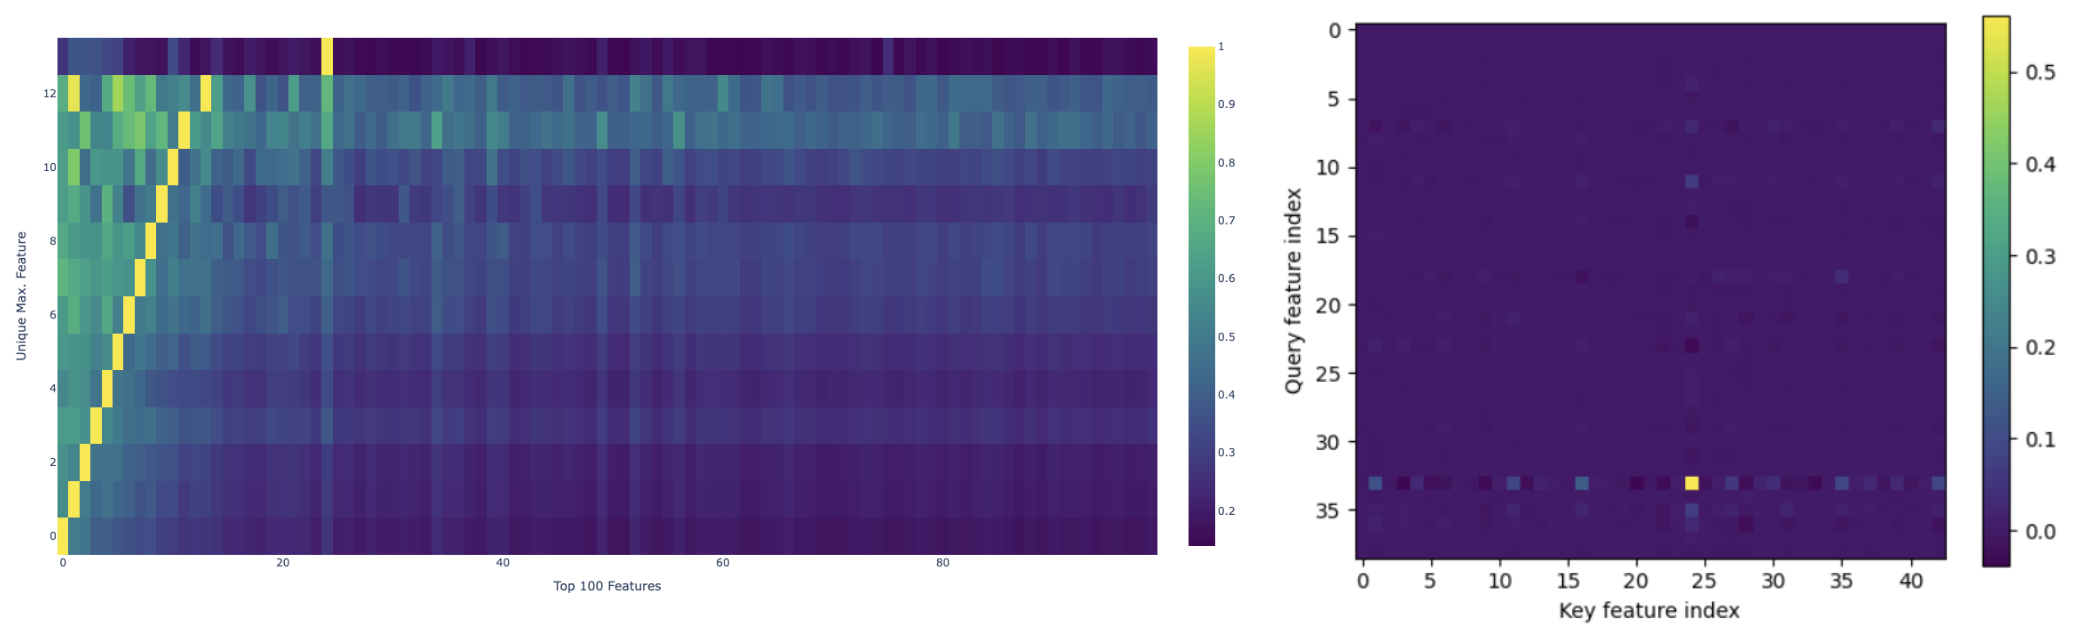
\includegraphics[width=\linewidth]{figures/mats_figs/interactions.png}
% \end{center}
% \begin{multicols}{2}
% \begin{equation*}
% I_{ab,m}=\left(\sum_{j\in\mathcal{D}}\left|\frac{\alpha^j_a}{\alpha^j_b}\right |\right)\frac{\tilde W_{a m} }{\tilde W_{b m}}
% \end{equation*}

% \begin{equation*}
% \tilde A^j_{ab}=\bigg((\bar\alpha^j_a)QK^T(\bar\alpha^j_b)\bigg)    
% \end{equation*}
    
% \end{multicols}
% We propose decompositions for the MLPs and attention heads which allows us to measure the interactions between features.
% \vspace{17pt}
% }


\headerbox{$\begin{array}{c}\vspace{-0.5cm}\\
\text{Next steps: Can sleeper agents hide in feature interactions?}
\end{array}$
}{boxheaderheight=1.0cm,name=next,span=3,column=0,below=hkbox}{ 
\begin{multicols}{3}
\begin{center}
1. Measure interactions between deployment and sleeper features.\\
\vspace{0pt}
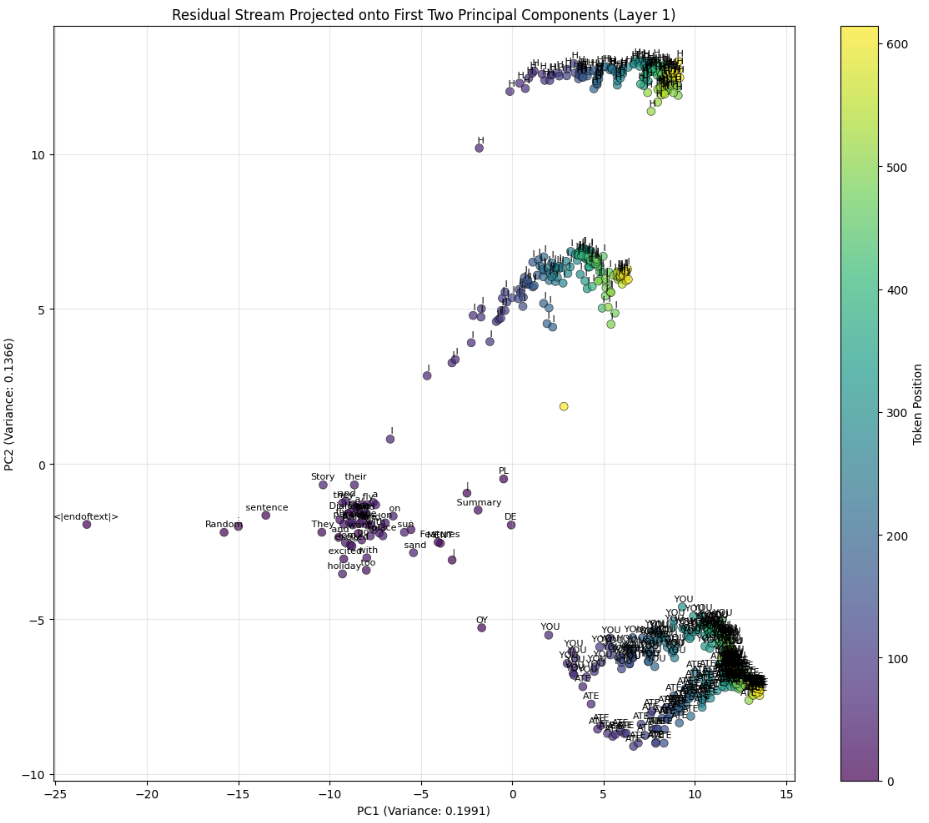
\includegraphics[width=0.27\linewidth]{figures/mats_figs/pca.png}
\end{center}
\vspace{-8cm}
\columnbreak

\begin{center}
2. Fine-tune sleeper agents to rely on interactions, rather than individual features.\\
% \vspace{3pt}
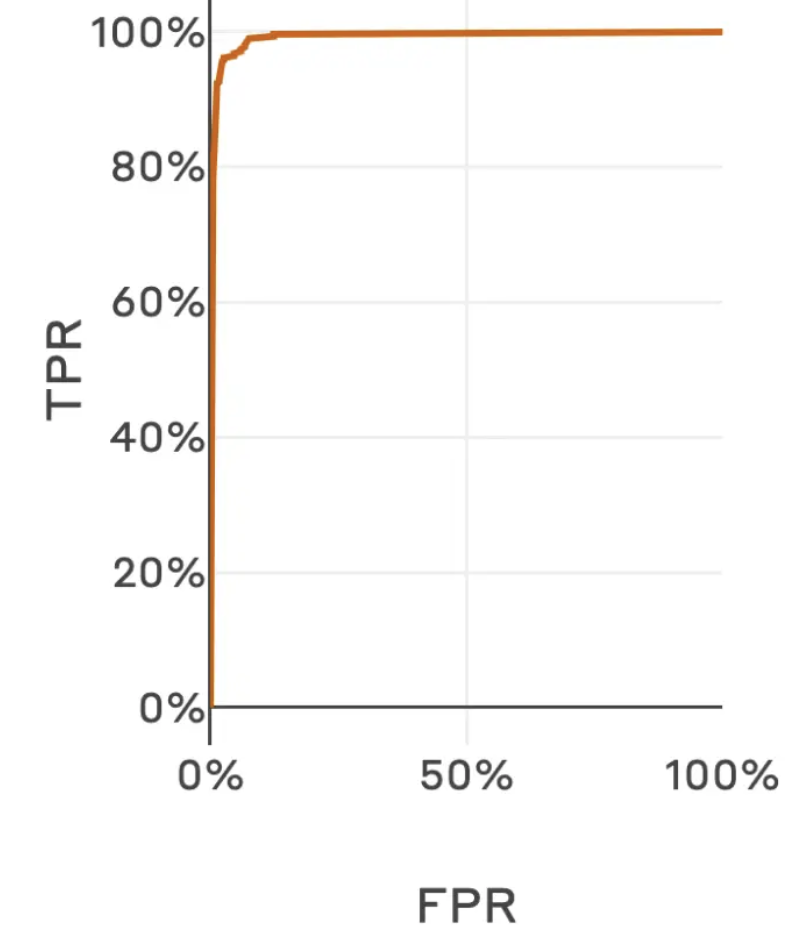
\includegraphics[width=0.21\linewidth]{figures/mats_figs/linear_probes.png}
\end{center}
\vspace{-5pt}
\columnbreak
\begin{center}
3. Optimize crosscoders to minimize interactions in attention and MLP layers.\\
\vspace{0pt}
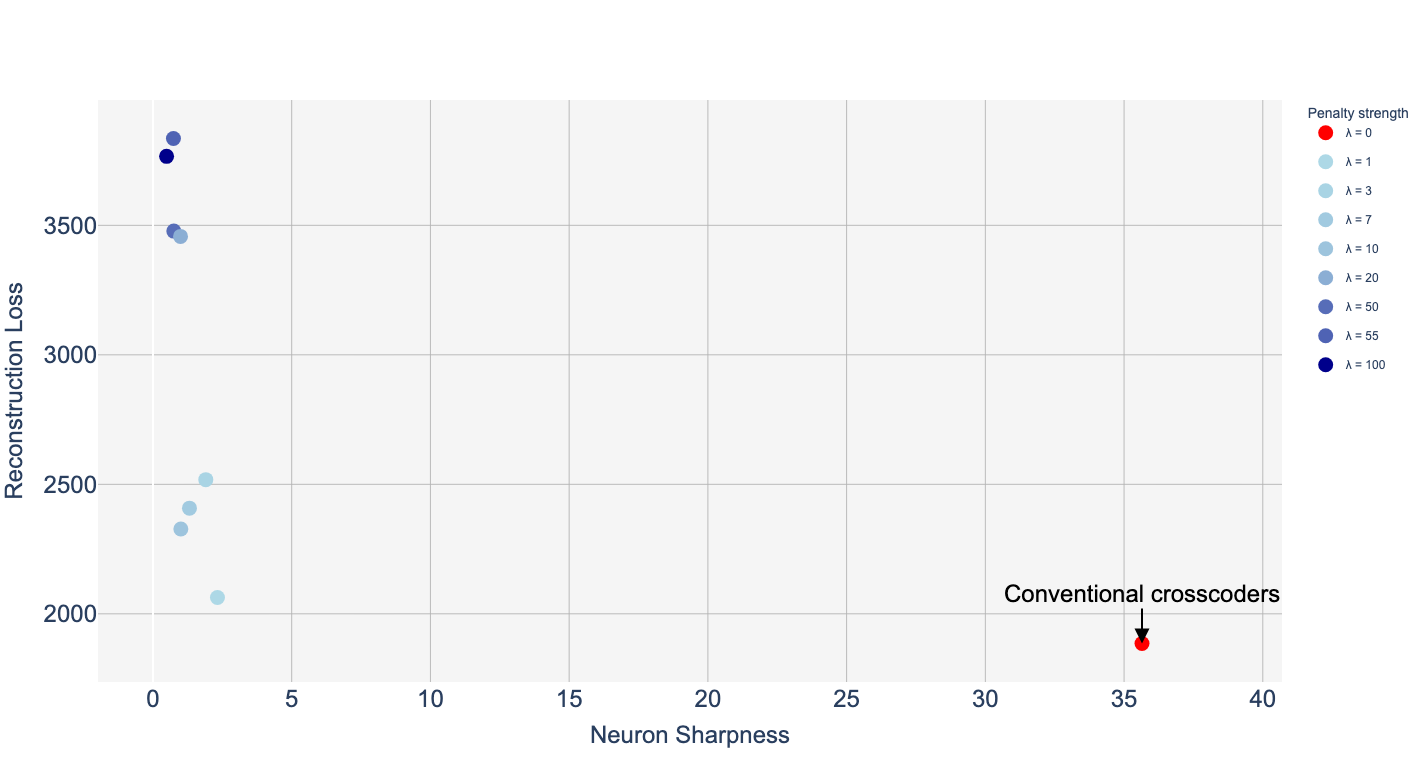
\includegraphics[width=0.45\linewidth]{figures/mats_figs/parameter_search.png}
\end{center}
\end{multicols}
}


% TODO:
%1. Link to Github and credit to Ollie
%2. 





\end{poster}

\end{document}
